%----------------------------------------------------------------------------------------------
%--------------------------------     3. Lineare Vektorräume    -------------------------------
%----------------------------------------------------------------------------------------------
\section{Lineare Vektorräume} 


%----------------------------------------------------------------------------------------------
%--------------------------------     3.1 Koordinatensystem    --------------------------------
%----------------------------------------------------------------------------------------------
\subsection{Koordinatensystem}

Ein Koordinatensystem ist festgelegt durch: 
\vspace{0.1cm}

\begin{itemize}
	\item Ursprung $O$
	\item Basis bestehend aus linear unabhängigen Basisvekoren \cbl{$b_i$}
\end{itemize}

\vspace{0.1cm}
\begin{tabular}{lll}
	Ortsvektor: & Vektor von Urspung zu Punkt	&  $\overrightarrow{OP} = \vec{p}= x \cdot \cbl{\vec{b}_1} + y \cdot \cbl{\vec{b}_2}$
\end{tabular}

\vspace{0.2cm}
$x$ und $y$ sind Koordinaten des Punktes $P$ bzw. Linearkombinationen der Basisvektoren \cbl{$b_i$}

$$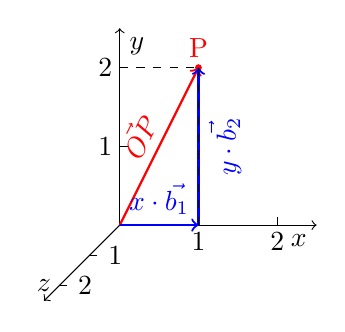
\begin{tikzpicture}

    % Draw axes
    \draw[->] (0,0,0) -- (2.5,0,0) node[anchor=north east]{$x$};
    \draw[->] (0,0,0) -- (0,2.5,0) node[anchor=north west]{$y$};
    \draw[->] (0,0,0) -- (0,0,2.5) node[anchor=south]{$z$};

    % Tick marks
    \foreach \x in {1,2} {
        \draw (\x,0,0) -- (\x,0.1,0) node[below=2pt] {$\x$};
    }
    \foreach \y in {1,2} {
        \draw (0,\y,0) -- (0.1,\y,0) node[left= 2pt] {$\y$};
    }
    \foreach \z in {1,2} {
        \draw (0,0,\z) -- (0.1,0,\z) node[right = 0.5pt] {$\z$};
    }

    % Draw a point
    \filldraw[red] (1,2,0) circle (1pt) node[anchor=south] {P};

    % Draw a vector v = (0.5,0.7,0.4)
    \draw[->, thick, red] (0,0,0) -- (1,2,0) node[midway, above, sloped] {$\vec{OP}$};
    \draw[->, thick, blue]  (0,0,0) -- (1,0,0) node[midway, above, sloped] {$x \cdot \vec{b_1}$};
    \draw[->, thick, blue]  (1,0,0) -- (1,2,0) node[midway, below, sloped] {$y \cdot \vec{b_2}$};

    
    % Optionally draw lines to axes
    \draw[dashed] (0,2,0) -- (1,2,0);
    \draw[dashed] (1,0,0) -- (1,2,0);
\end{tikzpicture}$$
		

%----------------------------------------------------------------------------------------------
%------------------------------------     3.2 Vektorraum    -----------------------------------
%----------------------------------------------------------------------------------------------
\subsection[Vektorraum]{Vektorraum  $\langle A \rangle$}		  

\begin{itemize}
	\item Menge aller Koordinaten (Linearkombinationen), welche durch die Vektoren $A = \vec{a}_1, \ldots , \vec{a}_n$ erreicht werden können.
	\item Durch bilden weiterer Linearkombinationen (Skalierungen) der Vektoren $\vec{a}_i$ verlässt man den Vektorraum nicht.
	\item Auch Additionen / Subtaktionen von Vektoren des Vektorraums verlassen den Verktorraum nicht.
\end{itemize}

\subsubsection{Dimension}

Die Dimension $\dim \langle A \rangle$ des Vektorraums besteht aus der maximalen Anzahl linear unabhängiger Vektoren im Vektorraum. 

\textrightarrow\ Linear abhängige Vektoren ändern die Dimension nicht!	
		

%----------------------------------------------------------------------------------------------
%-----------------------------     3.4 Basis eines Vektorraums    -----------------------------
%----------------------------------------------------------------------------------------------
\subsection{Basis eines Vektorraums}

Die Basis eines Vektorraus muss die folgenden Kriterien erfüllen:
\vspace{0.2cm}

\begin{enumerate}
	\item Lineare Unabhängigkeit der Basisvektoren \cbl{$\vec{b}_i$}, damit Koordinaten \cor{$x_i$} eindeutig sind 
	\item Basisvektoren \cbl{$\vec{b}_i$} müssen den ganzen Vektorraum aufspannen
\end{enumerate}


\example{Punkt mittels Basisvektoren beschreiben}

$$ \vec{p} = \cor{x_1} \cdot \cbl{\vec{b}_1} + \cor{x_2} \cdot \cbl{\vec{b}_2} + \cor{x_3} \cdot \cbl{\vec{b}_3}  
= \cbl{B} \cor{x} =
\begin{pmatrix}
	1 & 0 & 0 \\
	0 & 1 & 0 \\ 
	0 & 0 & 1
\end{pmatrix}
\begin{pmatrix}
	x_1 \\ x_2 \\ x_3
\end{pmatrix} $$

$\vec{b}_1$, $\vec{b}_2$ und $\vec{b}_3$ sind im Beispiel die Standardbasisvektoren. 
Es können aber auch irgendwelche Vektoren einer anderen Basis sein.


%----------------------------------------------------------------------------------------------
%-------------------------------     3.5 Lineare Abbildungen    -------------------------------
%----------------------------------------------------------------------------------------------
\subsection{Lineare Abbildungen (Bilder des Vektoraums)}

Eine lineare Abbildung: 
\vspace{0.1cm}

\begin{itemize}
	\item bildet Geraden auf Geraden ab
	\item erhält Parallelität
	\item fixiert den Ursprung
\end{itemize}

\vspace{0.2cm}

Lineare Abbildungen werden mit der Abbildungsmatrix $A$ beschrieben.
\vspace{0.1cm}
\begin{itemize}
	\item \textbf{Die Spalten von A sind Bilder der Basisvektoren}
	\item Eine Abbildung $A$ kann durch ihre \textbf{Inverse} $A^{-1}$ rückgängig gemacht werden.
\end{itemize}


\example{Abbildungsmatrix $A$ einer Scherung}

\begin{minipage}[c]{0.5\columnwidth}
	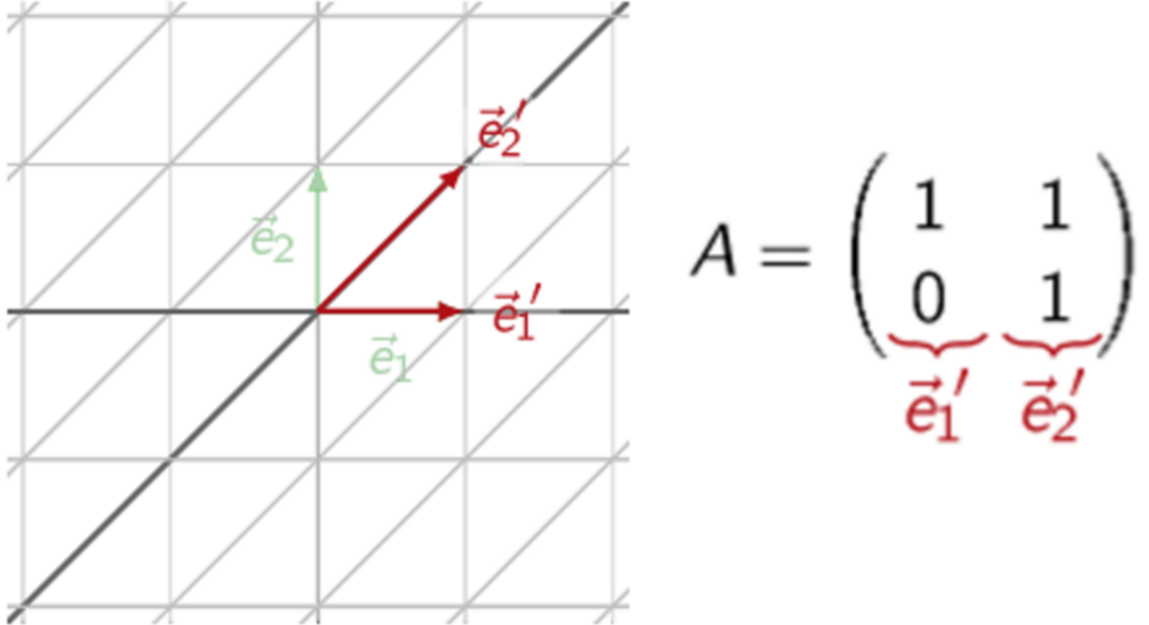
\includegraphics[width=\columnwidth]{images/scherung.PNG}
\end{minipage}
\hfill
\begin{minipage}[c]{0.48\columnwidth}
	Die Standardbasisvektoren $\vec{e}_1$ und $\vec{e}_2$ werden durch die Abbildungsmatrix $A$ auf die Vektoren $\vec{e}_1'$ und $\vec{e}_2'$ abgbildet.

	Die Spalten der Abbildungsmatrix $A$ enthalten die Bilder $\vec{e}_1'$ und $\vec{e}_2'$ der Standardbasisvektoren $\vec{e}_1$ und $\vec{e}_2$
\end{minipage}


\subsubsection{Anwendung einer Abbildung auf einen Vektor}

Der Vektor $\vec{v}$ wird mit der Abbildungsmatrix auf den Vektor $\vec{v'}$ abgebildet:
$$ A \cdot \vec{v} = \vec{v'}$$		

Die Abbildung kann mittels $A^{-1} \cdot \vec{v'} = \vec{v}$ rückgängig gemacht werden.

\textbf{\textrightarrow\ Das geht nur, wenn A eine quadratische Matrix ist!}


\subsubsection{Zusammensetzung linearer Abbildungen}

Wenn mehrere lineare Abbildungen 'wirken', so werden die Abbildngsmatritzen multipliziert.

\textbf{Die als erstes wirkende Abbildung steht dabei ganz rechts in der Multiplikation!}


\example{Zusammensetzung linearer Abbildungen}
\vspace{-0.2cm}
$$ \text{Abbildungsmatrix:} C = AB \qquad \text{\textrightarrow\ Erst wirkt Abbildungsmatrix $B$, danach $A$} $$ 


%----------------------------------------------------------------------------------------------
%-----------------------     3.6 Basiswechsel für lineare Abbildungen    ----------------------
%----------------------------------------------------------------------------------------------
\subsection{Basiswechsel für lineare Abbildungen}

Die lineare Abbildung, die in der Basis $B$ durch die Matrix $A$ beschrieben wird, wird in der Basis $C$ durch die Matrix $A'$ beschrieben.
		
\begin{minipage}{0.6\columnwidth}
	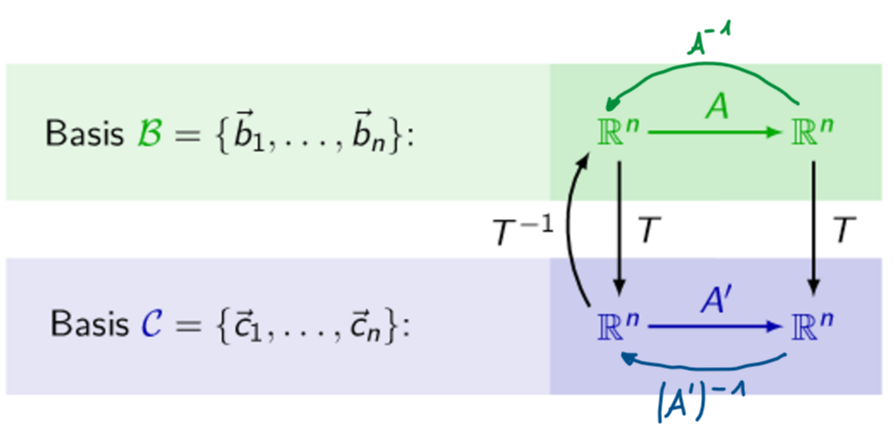
\includegraphics[width=\columnwidth]{images/basiswechsel_abbildungen.PNG}
\end{minipage}						
\hfill
\begin{minipage}{0.35\columnwidth}
		\begin{align*}
			\cbl{A'} &= T \cgn{A} \,T^{-1} 		\\
			\det(A') &= \det(A)					\\
			\text{Spur}(A') &= \text{Spur}(A)	\\
		\end{align*}
\end{minipage}


%----------------------------------------------------------------------------------------------
%--------------------------     3.7 Elementare Abbildungsmatritzten    ------------------------
%----------------------------------------------------------------------------------------------
\subsection{Elementare Abbildungsmatritzten}

\subsubsection{Drehmatrix $D$ finden}

Die Drehung wird beschrieben durch $D \cdot A = A'$	\\
Die Spalten der Matrix $A$ sind die Punkte vor der Drehung, $A'$ enthält die Punkte nach der Drehung (Bilder)
$D = A' \cdot A^{-1}$ 

\textbf{Die Matritzten müssen quadratisch sein! Falls nötig Matritzen mit einem Punkt erweitern, damit sie quadratisch werden}
		
		
\subsubsection{Spiegelungen (orthogonale Matrix)}

\vspace{-0.2cm}
$$ \det(A) = -1 $$

\textbf{2 Dimensionen:}
\vspace{0.2cm}
\begin{tabular}{ccc}
	$x$-Achse & $y$-Achse & an 45° Geraden \\
	
	$\begin{pmatrix} 1 & 0 \\ 0 & -1 \end{pmatrix}$ & $\begin{pmatrix} -1 & 0 \\ 0 & 1 \end{pmatrix}$ & $\begin{pmatrix} 0 & 1 \\ 1 & 0 \end{pmatrix}$
\end{tabular}

\vspace{0.2cm}

\textbf{3 Dimensionen:}
\vspace{0.2cm}
\begin{tabular}{ccc}
	$xy$-Ebene & $xz$-Ebene & an $yz$-Ebene\\
	$\begin{pmatrix} 1 & 0 & 0 \\ 0 & 1 & 0 \\ 0 & 0 & -1 \end{pmatrix}$ & $\begin{pmatrix} 1 & 0 & 0 \\ 0 & -1 & 0 \\ 0 & 0 & 1 \end{pmatrix}$ & $\begin{pmatrix} -1 & 0 & 0 \\ 0 & 1 & 0 \\ 0 & 0 & 1 \end{pmatrix}$ \\
\end{tabular}		  	
\vspace{0.2cm}	


\subsubsection{Projektionen}		

Projektionen auf etwas (z.B. die Koordinatenachsen) liefern die 'Länge des Schattens' des Vektors auf diese Achse. \qquad $P^2 = P$ 
\vspace{0.2cm}

\textbf{2 Dimensionen:}
\vspace{0.2cm}
\begin{tabular}{cc}
	$x$-Achse & $y$-Achse \\
	$\begin{pmatrix} 1 & 0  \\ 0 & 0  \end{pmatrix}$ & $\begin{pmatrix} 0 & 0  \\ 1 & 0  \end{pmatrix}$
\end{tabular}				
	
\vspace{0.2cm}

\textbf{3 Dimensionen:}
\vspace{0.2cm}
\begin{tabular}{ccc}
	$xy$-Ebene & $xz$-Ebene & an $yz$-Ebene\\
	$\begin{pmatrix} 1 & 0 & 0 \\ 0 & 1 & 0 \\ 0 & 0 & 0 \end{pmatrix}$ & $\begin{pmatrix} 1 & 0 & 0 \\ 0 & 0 & 0 \\ 0 & 0 & 1 \end{pmatrix}$ & $\begin{pmatrix} 0 & 0 & 0 \\ 0 & 1 & 0 \\ 0 & 0 & 1 \end{pmatrix}$
\end{tabular}		  	
\vspace{0.2cm}


\subsubsection{Drehungen $D$ (orthogonale Matrix)}

Die Spalten von $D_{\alpha}$ sind Bilder der Basisvektoren 

Determinante: \quad $\det(D) = 1$

\vspace{0.2cm}
\begin{itemize}
	\item Die Drehung findet \textbf{gegen den Uhrzeigersinn} statt 
	\item Für Drehung in Uhrzeigersinn: $D_{-\alpha} = D_{\alpha}^{-1}$ verwenden \textrightarrow\ $D_{\alpha} D_{\beta} = D_{\alpha + \beta}$
\end{itemize}

\vspace{0.3cm}
	  	
\textbf{2 Dimensionen:} 
\quad
$D_{\alpha} = \begin{pmatrix} \cos(\alpha) & -\sin(\alpha)  \\ \sin(\alpha) & \cos(\alpha)  \end{pmatrix}$

\textbf{3 Dimensionen} 
\vspace{0.2cm}

\begin{tabular}{cc}
	Drehung um $x$-Achse & Drehung um $y$-Achse \\
	$D_{x} = \begin{pmatrix} 1 & 0 & 0 \\
	0 & \cos(\alpha) & -\sin(\alpha)  \\ 0 & \sin(\alpha) & \cos(\alpha)  \end{pmatrix}$ & $D_{y} = \begin{pmatrix} \cos(\alpha) & 0 & \sin(\alpha) \\
	0 & 1 & 0 \\ -\sin(\alpha) & 0 & \cos(\alpha)  \end{pmatrix}$\\
	\\
	Drehung um $z$-Achse & \\
	$D_{z} = \begin{pmatrix} \cos(\alpha) & -\sin(\alpha) & 0 \\ \sin(\alpha) & \cos(\alpha) & 0 \\ 0 & 0 & 1 \end{pmatrix}$
\end{tabular}

\subsection{Spur}	
\label{Spur}	  	

Die Spur einer Matrix ist die Summe der Elemente auf der Diagonalen
\vspace{0.2cm}

\begin{minipage}[t]{0.2\columnwidth}
	$A = 
	\begin{pmatrix}
		\cbl{1} & 7 & 9 \\
		2 & \cbl{9} & 6 \\ 
		8 & 3 & \cbl{5}	
	\end{pmatrix}$
\end{minipage}
\hfill
\begin{minipage}[t]{0.7\columnwidth}
	$\mathrm{Spur}(A) = \cbl{1} + \cbl{9} + \cbl{5} = 15$ 
\end{minipage}

\vspace{0.3cm}

\subsubsection{Rechenregeln Spur}

\begin{tabular}{llclcl}
	Vertauschung 			& Spur$(BA)$ & $=$  & Spur$(AB)$ \\
	Zyklische Vertauschung:	& Spur$(ABC)$ & $=$ & Spur$(CAB)$ &  $=$ & Spur$(BCA)$ \\
	Anwendung: 				& Spur$(TAT^{-1})$ & $=$ & Spur$(T^{-1}TA)$ & $=$ & Spur$(A)$
\end{tabular}
